\chapter{Background}
\minitoc

\section{Recommendation Systems}\label{sec:recommendation-systems}
A recommendation system is an artificial intelligence (AI) technology that provides users with recommendations for items that they may be interested in using Big Data and machine learning techniques. 

Recommender systems undergo training to understand the preferences, earlier decisions, and attributes of the user and products using their past interactions which includes impressions, clicks, purchases, and ratings. Recommender systems are usually used by content and product providers to suggest items to users that they may like based on their profile and preferences. 

\section{Types of Recommendation Systems}\label{sec:types-of-recommendation-systems}
\subsection{Classical recommendation systems}\label{subsec:classical-recommendation-systems}
\begin{itemize}
    \item \textbf{Collaborative Filtering} \\ Collaborative Filtering is a technique that can filter out items that a user might like on the basis of reactions by similar users. It works by searching a large group of people and finding a smaller set of users with tastes similar to a particular user. It looks at the items they like and combines them to create a ranked list of suggestions. This technique is based on the idea that people who agreed in the past will agree in the future.
    \begin{figure}[H]
        \centering
        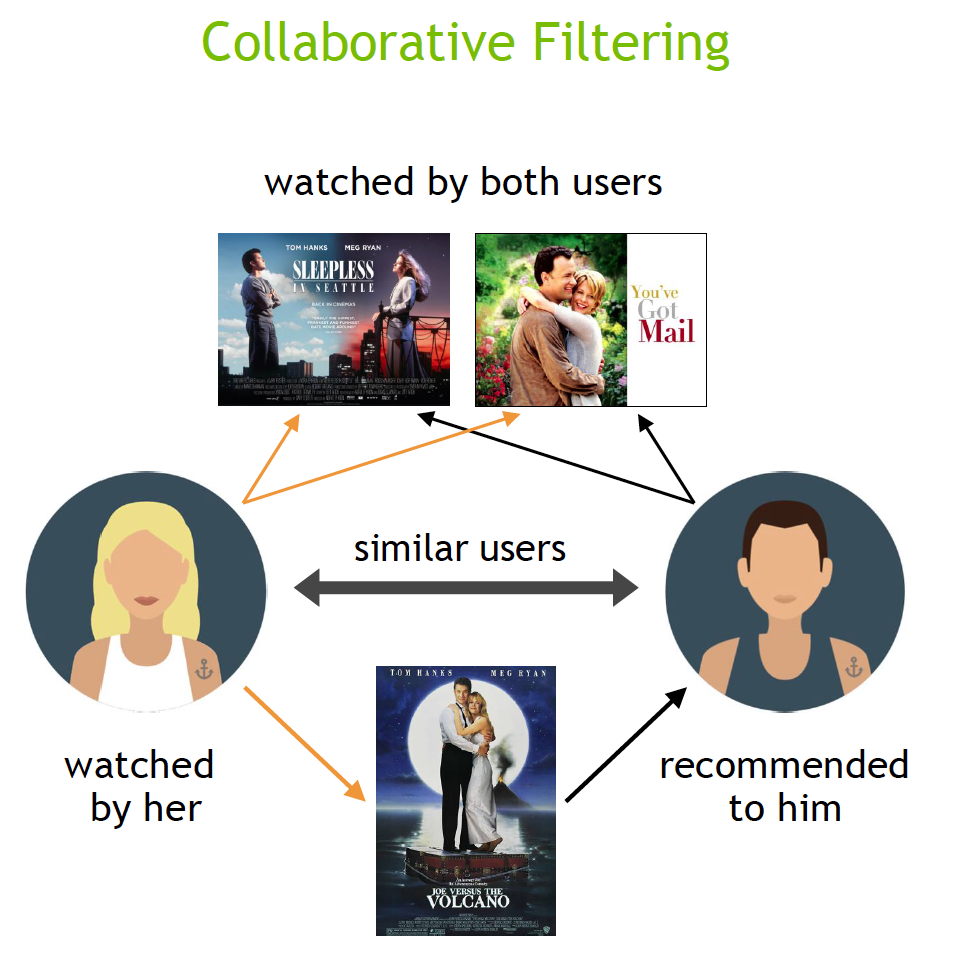
\includegraphics[width=0.4\textwidth]{assets/collaborative_filtering.png}
        \caption{Collaborative Filtering}
        \label{fig:collaborative-filtering}
        \cite{NvidiaRecSys}
    \end{figure}
    \item \textbf{Content Filtering}\\Content Filtering is a technique that uses the features of items a user has interacted with in order to recommend additional items with similar properties. This technique is based on the idea that if a user liked a particular item, he or she will also like an item that is similar to it. 
    \begin{figure}[H]
        \centering
        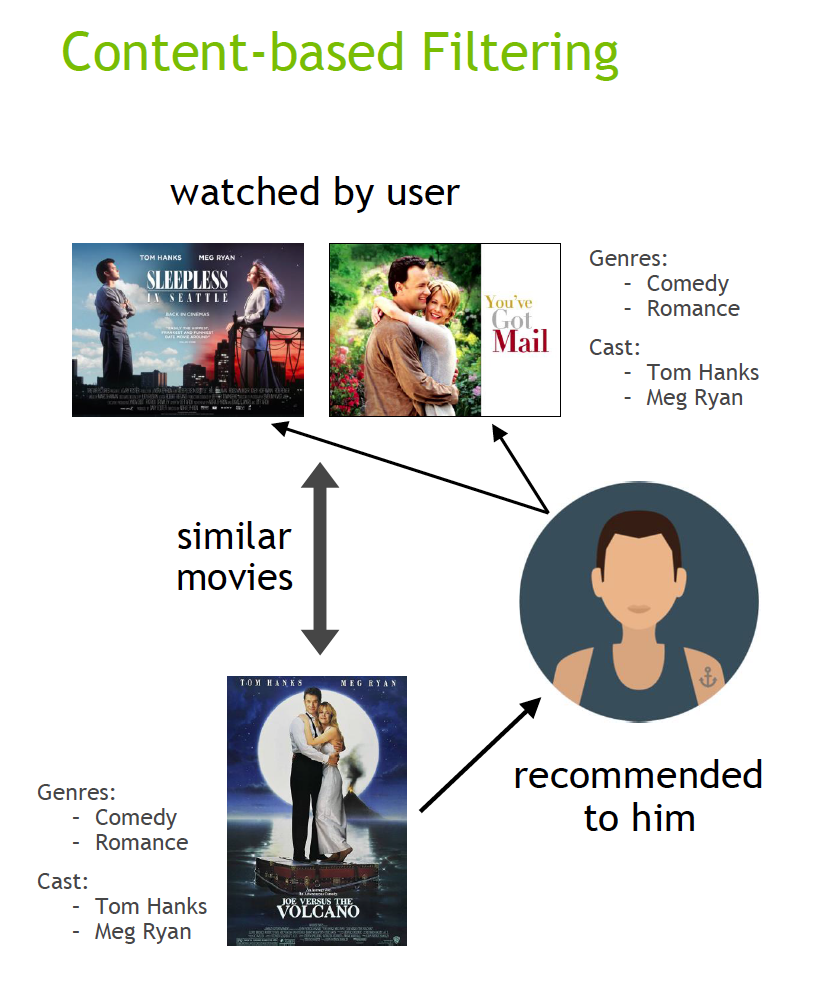
\includegraphics[width=0.4\textwidth]{assets/content_based_filtering.png}
        \caption{Content Filtering}
        \label{fig:content-filtering}
        \cite{NvidiaRecSys}
    \end{figure}
    \item \textbf{Hybrid Recommendation Systems}\\Hybrid Recommendation Systems combine the advantages of the types above to create a more comprehensive recommending system.
    \item \textbf{Context Filtering}\\Context Filtering is a technique that uses the contextual information of the user by framing the recommendation problem as a contextual multi-armed bandit problem and using the contextual information to learn the user's preferences.
    \begin{figure}[H]
        \centering
        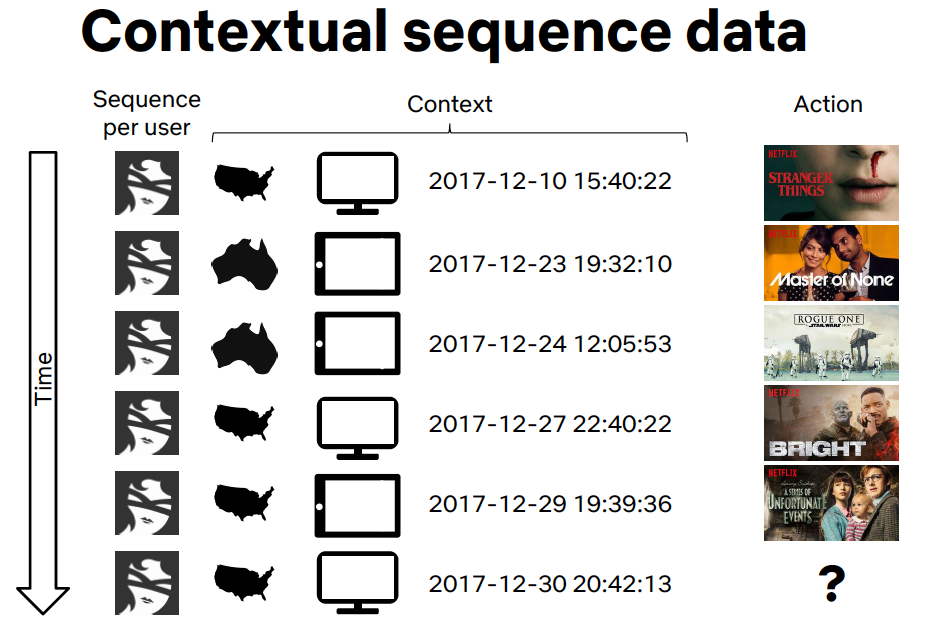
\includegraphics[width=0.4\textwidth]{assets/contextual-sequence-prediction.png}
        \caption{Context Filtering}
        \label{fig:costextual-filtering}
        \cite{NvidiaRecSys}
    \end{figure}
\end{itemize}

\subsection{Deep learning-based recommendation systems}\label{subsec:deep-learning-based-recommendation-systems}
These systems use deep learning techniques to learn the user's preferences and recommend items.
\begin{itemize}
    \item \textbf{Neural Collaborative Filtering}\\Neural Collaborative Filtering is a technique that uses neural networks to learn the user's preferences and recommend items. It uses a neural network to learn the user's preferences and a neural network to learn the item's features. The two networks are then combined to create a recommendation.
    \begin{figure}[H]
        \centering
        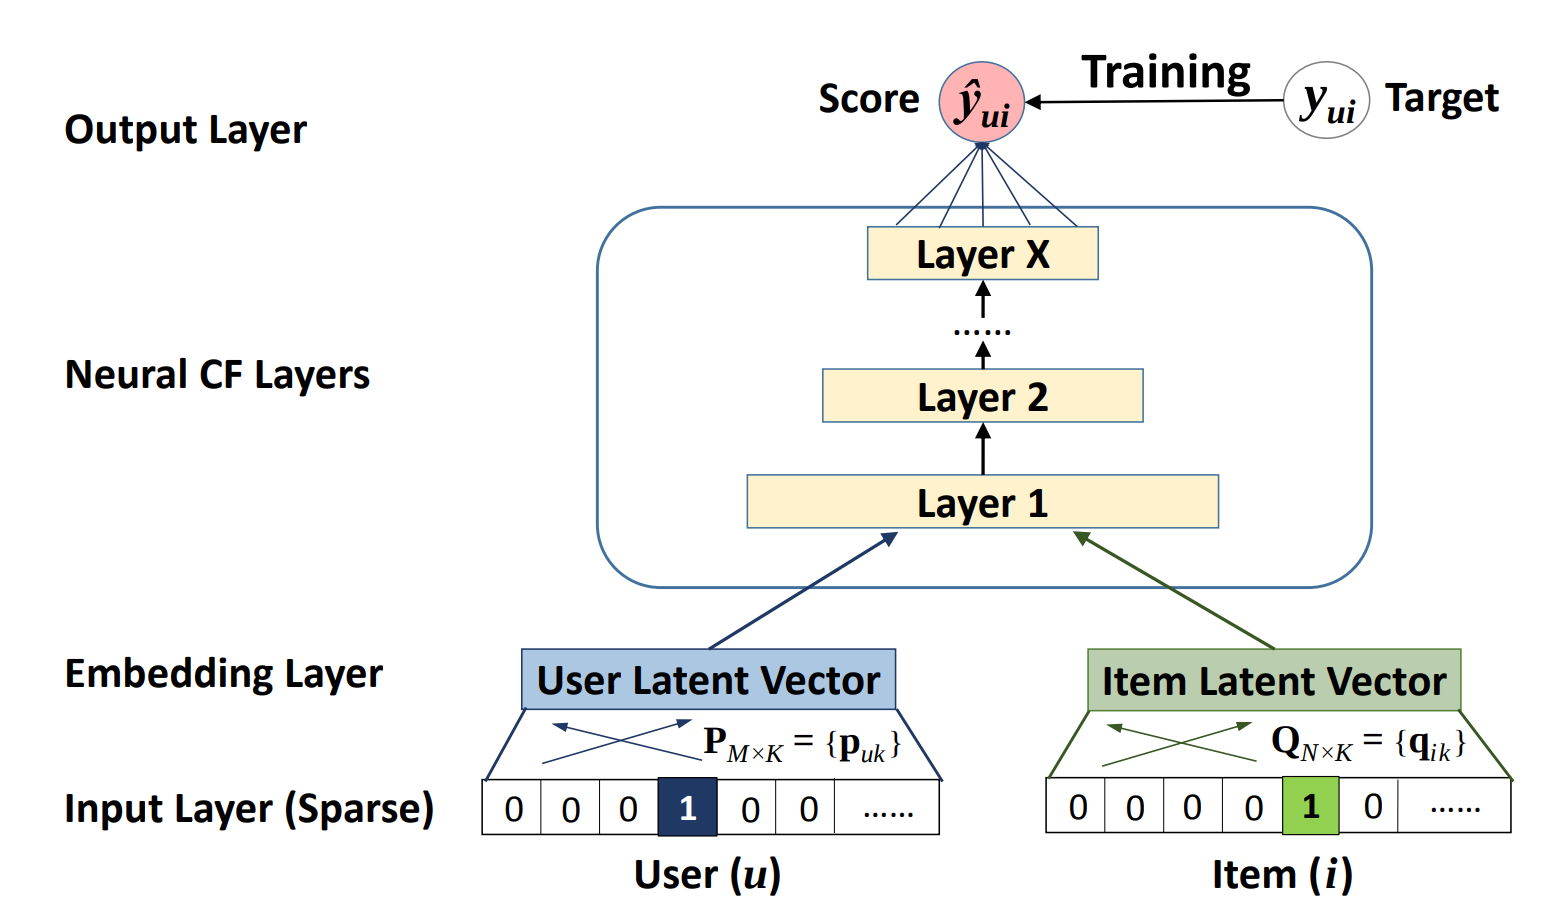
\includegraphics[width=0.4\textwidth]{assets/neural-collaborative-filtering.png}
        \caption{Neural Collaborative Filtering}
        \label{fig:neural-collaborative-filtering}
        \cite{NvidiaRecSys}
    \end{figure}
    \item \textbf{Variational Autoencoder for Collaborative Filtering}\\This model consists of two parts: an encoder and a decoder. The encoder takes the user's preferences as input and encodes them into a latent space. The decoder takes the latent space as input and decodes it into the item's features.
    \begin{figure}[H]
        \centering
        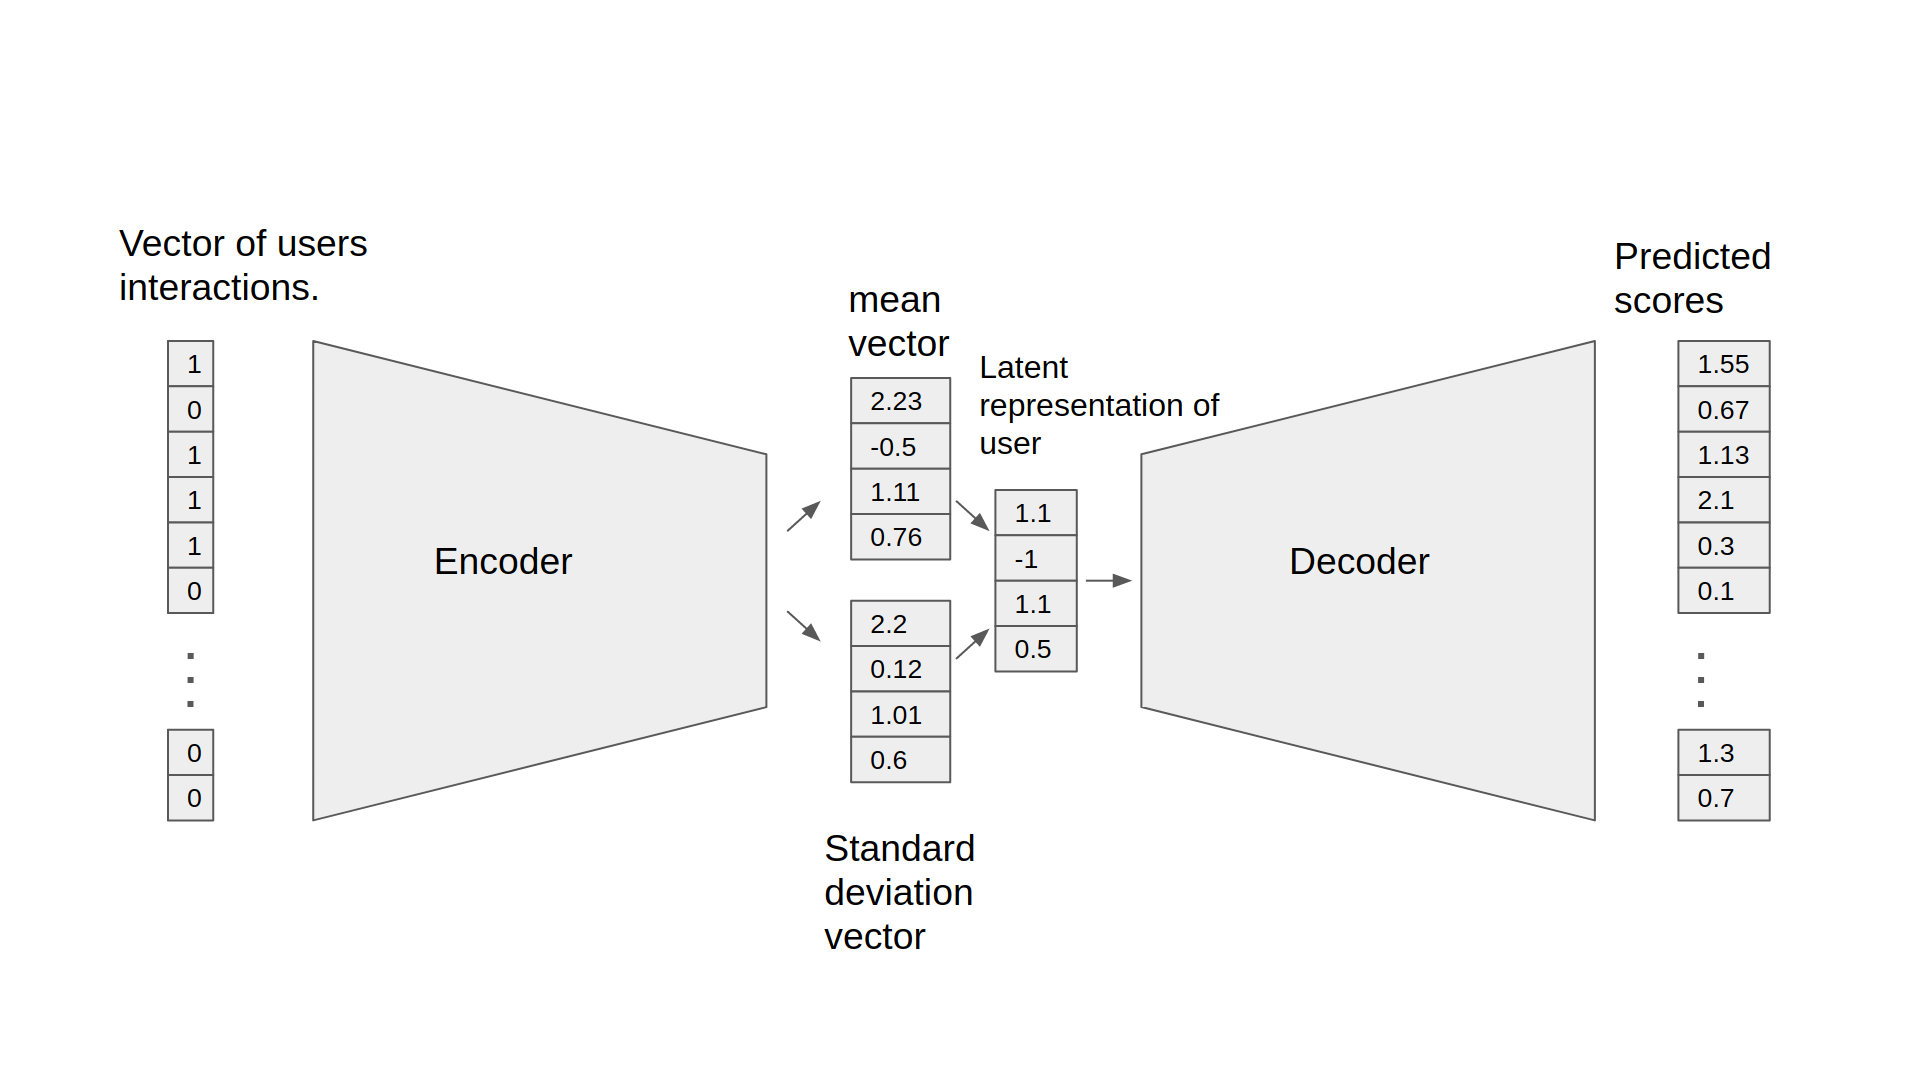
\includegraphics[width=0.4\textwidth]{assets/variational-autoencoder.png}
        \caption{Variational Autoencoder for Collaborative Filtering Structure}
        \label{fig:variational-autoencoder-for-collaborative-filtering}
        \cite{NvidiaRecSys}
    \end{figure}
    \item \textbf{Contextual Sequence Learning} \\ Contextual Sequence Learning is a technique that uses a recurrent neural network to learn the user's preferences and a neural network to learn the item's features. The two networks are then combined to create a recommendation.
    \item \textbf{Wide \& Deep} \\ Wide \& Deep is a technique that uses a wide neural network to learn the user's preferences and a deep neural network to learn the item's features. The wide model is generalized linear model (GLM) and the deep model is a dense neural network (DNN).
    \item \textbf{DLRM} \\ Deep Learning Recommendation Model (DLRM) it is a technique that uses a deep neural network to handle categorical and numerical features. each categorical feature is represented as a one-hot vector and each numerical feature is represented as a dense vector, both fed into multi-layer perceptron (MLP) layers. The output of the MLP layers is then fed into a dot product layer to compute the inner product of the feature vectors. The output of the dot product layer is then fed into a sigmoid layer to compute the probability of the user liking the item.
    \begin{figure}[H]
        \centering
        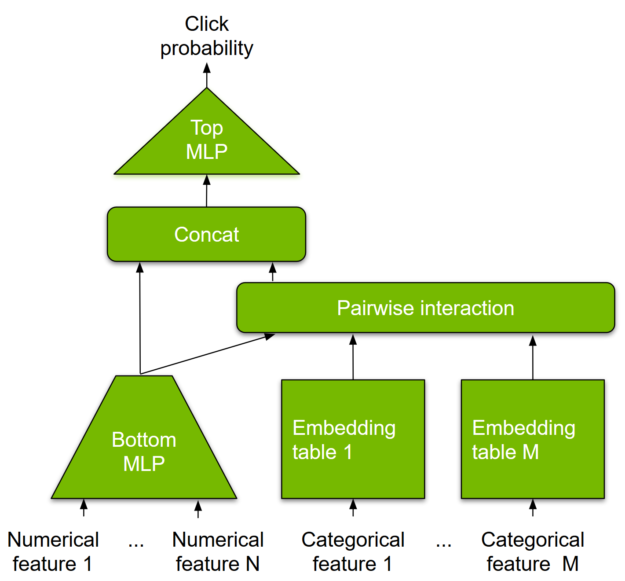
\includegraphics[width=0.4\textwidth]{assets/dlrm.png}
        \caption{DLRM Structure}
        \label{fig:dlrm}
        \cite{NvidiaRecSys}
    \end{figure}
\end{itemize}